\documentclass[12pt,twoside]{mitthesis-exec}

%%%%%%%%%%%%%%%%%%%%%%%%%%%%%%%%%%%%%%%%%%%%%%%%%%%%%%%%%%%%%%%%%%%%%%%%%%%%%%%%
% PREAMBLE

\usepackage[bitstream-charter]{mathdesign} % Use BT Charter font
\usepackage[T1]{fontenc}                   % Use T1 encoding instead of OT1
\usepackage[utf8]{inputenc}                % Use UTF8 input encoding
\usepackage{microtype}                     % Improve typography
\usepackage{amsmath}                       % AMS Math extensions
\usepackage{booktabs}                      % Improve table spacing
\usepackage{graphicx}                      % Extended graphics capabilities
\usepackage{tocbibind}                     % Include listings in TOC
\usepackage[printonlyused]{acronym} % withpage: for showing page of use
\usepackage{listings}                      % Source code listings
\usepackage{caption}
\usepackage{subcaption}
\usepackage[rgb]{xcolor}
\usepackage{url}
\usepackage{soul}
\usepackage{array}
\usepackage{pdfpages}
\usepackage{mathtools}
\usepackage{setspace}
\usepackage{pbox}
\usepackage{tikz}
\usetikzlibrary{calc,shapes,decorations.pathreplacing,positioning}
\usepackage{pgfplots}

\usepackage[breaklinks=true]{hyperref}
\hypersetup{colorlinks=true, linkcolor=black, citecolor=black, urlcolor=black,
  pdftitle={Domain Decomposition for Monte Carlo Particle Transport Simulations
  of Nuclear Reactors},
  pdfauthor={Nicholas E. Horelik}
}
\pagestyle{plain}

%\usepackage{floatrow}
%\floatsetup[table]{style=plaintop}
%\floatsetup[widefigure]{margins=hangleft}

% Appendix
\usepackage[toc,page]{appendix}

% Don't reset footnote counter between chapters
\usepackage{chngcntr}
\counterwithout{footnote}{chapter}

% Algorithm constructs
\usepackage[chapter]{algorithm} % Provides algorithm environment
\usepackage{algorithmicx}       % Provides algorithmic block
\usepackage{algpseudocode}      % Option of algorithmicx package
\renewcommand{\thealgorithm}{\thechapter-\arabic{algorithm}}
\newcommand\Algphase[1]{%
\vspace*{-.7\baselineskip}\Statex\hspace*{\dimexpr-\algorithmicindent-2pt\relax}\rule{\columnwidth}{0.4pt}%
\Statex\hspace*{-\algorithmicindent}{#1}%
\vspace*{-.7\baselineskip}\Statex\hspace*{\dimexpr-\algorithmicindent-2pt\relax}\rule{\columnwidth}{0.4pt}%
}
\newcommand{\algrule}[1][.4pt]{\par\vskip.5\baselineskip\hrule height #1\par\vskip.5\baselineskip}

% Configure captions
\captionsetup{labelfont=bf, labelsep=colon}
\captionsetup[algorithm]{labelfont=bf, labelsep=colon}

% Use Latin Modern for typewriter fonts
\renewcommand{\ttdefault}{lmtt}

% Add \unit macro
\newcommand{\unit}[1]{\ensuremath{\, \mathrm{#1}}}

\definecolor{gray}{rgb}{0.4,0.4,0.4}
\definecolor{darkblue}{rgb}{0.0,0.0,0.6}
\definecolor{cyan}{rgb}{0.0,0.6,0.6}
\lstset{
  basicstyle=\footnotesize\ttfamily,
  columns=fullflexible,
  showstringspaces=false,
  commentstyle=\color{gray}\upshape,
  frame=single,
  xleftmargin=0.55in
}

\lstdefinelanguage{XML}
{
  morestring=[b]",
  morestring=[s]{>}{<},
  morecomment=[s]{<?}{?>},
  morecomment=[s]{<!--}{-->},
  stringstyle=\color{black},
  identifierstyle=\color{darkblue},
  keywordstyle=\color{cyan},
  morekeywords={}
}

\setcounter{secnumdepth}{4}
\setcounter{tocdepth}{3}

\renewcommand{\contentsname}{Table of Contents}
\renewcommand{\bibname}{References}

\makeatletter \renewcommand\thealgorithm{\arabic{algorithm}} \@addtoreset{algorithm}{chapter} \makeatother

\begin{document}

%%%%%%%%%%%%%%%%%%%%%%%%%%%%%%%%%%%%%%%%%%%%%%%%%%%%%%%%%%%%%%%%%%%%%%%%%%%%%%%%
% TITLE PAGE

\title{EXECUTIVE SUMMARY \\~\\ Domain Decomposition for Monte Carlo Particle
Transport Simulations of Nuclear Reactors}

\author{Nicholas E. Horelik}
\prevdegrees{B.S., Tufts University(2009) \\
             M.S., Massachusetts Institute of Technology (2012)}
\department{Department of Nuclear Science and Engineering}
\degree{Doctor of Philosophy in Nuclear Science and Engineering}

\degreemonth{February}
\degreeyear{2014}
\thesisdate{January 15, 2014}

\supervisor{Benoit Forget}{Associate Professor of Nuclear Science and
  Engineering}
\supervisor{Kord S. Smith}{KEPCO Professor of the Practice of Nuclear Science and
  Engineering}
\chairman{Mujid S. Kazimi}{TEPCO Professor of Nuclear Engineering \\ Chairman,
  Department Committee on Graduate Students}

%%%%%%%%%%%%%%%%%%%%%%%%%%%%%%%%%%%%%%%%%%%%%%%%%%%%%%%%%%%%%%%%%%%%%%%%%%%%%%%%
%%%%%%%%%%%%%%%%%%%%%%%%%%%%%%%%%%%%%%%%%%%%%%%%%%%%%%%%%%%%%%%%%%%%%%%%%%%%%%%%
% ABSTRACT

\setcounter{savepage}{\thepage}

\begin{abstractpage}

The development of high fidelity multi-group neutron transport-based simulation tools for full core Light Water Reactor (LWR) analysis has been a long-standing goal of the reactor physics community. While direct transport simulations have previously been far too computationally expensive, advances in computer hardware have allowed large scale simulations to become feasible. Therefore, many have focused on developing full core neutron transport solvers that do not incorporate the approximations and assumptions of traditional nodal diffusion solvers. 

Due to the computational expense of direct full core 3D deterministic neutron transport methods, many have focused on 2D/1D methods which solve 3D problems as a coupled system of radial and axial transport problems. However, the coupling of radial and axial problems also introduces approximations. Instead, the work in this thesis focuses on explicitly solving the 3D deterministic neutron transport equations with the Method of Characteristics (MOC).

MOC has been widely used for 2D lattice physics calculations due to its ability to accurately and efficiently simulate reactor physics problems with explicit geometric detail. The work in this thesis strives to overcome the significant computational cost of solving the 3D MOC equations by implementing efficient track generation, axially extruded ray tracing, Coarse Mesh Finite Difference (CMFD) acceleration, linear track-based source approximations, and scalable domain decomposition. 

Additionally, significant attention has been be given to complications that arise in full core simulations with transport-corrected cross-sections. The convergence behavior of transport methods is analyzed, leading to a new strategy for stabilizing the source iteration scheme for neutron transport simulations. The methods are incorporated into the OpenMOC reactor physics code and simulation results are presented for the full core BEAVRS LWR benchmark. Parameter refinement studies and comparisons with reference OpenMC Monte Carlo solutions show that converged full core 3D MOC simulations are feasible on modern supercomputers for the first time.

%However, 3D full core LWR simulations present significant challenges due to greatly increased computational cost.

%The Method of Characteristics (MOC) has seen wide interest in reactor physics because of its accuracy and efficiency in computing lattice physics problems. While most of its use has been in solving 2D problems, there has been recent interest in extending MOC to 3D in order to more accurately calculate 3D power distributions in LWRs. While the method is naturally extensible to 3D, it presents significant computational difficulties. Methods will be presented which mitigate the computational difficulties of 3D MOC by using domain decomposition, efficient track generation, axially extruded ray tracing, CMFD acceleration, and a linear source approximation. Significant attention will be given to complications that arise in full core simulations. 3D MOC results will be presented for the full core simulation of the BEAVRS benchmark, showing that 3D MOC can be a viable tool for anal

\end{abstractpage}

\singlespacing 

%%%%%%%%%%%%%%%%%%%%%%%%%%%%%%%%%%%%%%%%%%%%%%%%%%%%%%%%%%%%%%%%%%%%%%%%%%%%%%%%
%%%%%%%%%%%%%%%%%%%%%%%%%%%%%%%%%%%%%%%%%%%%%%%%%%%%%%%%%%%%%%%%%%%%%%%%%%%%%%%%
\section*{Introduction}

%%%%%%%%%%%%%%%%%%%%%%%%%%%%%%%%%%%%%%%%%%%%%%%%%%%%%%%%%%%%%%%%%%%%%%%%%%%%%%%%
\subsection*{Background and Motivation}

We desire higher-fidelity simulations of full nuclear reactor systems to
help us better understand the current fleet of aging reactors, as well as better
evaluate new designs. One option for solving for neutron distributions is with
\textbf{Monte Carlo} (MC) methods.

\begin{itemize}
  \item MC methods provide the highest-quality solutions by sampling directly from
  evaluated nuclear data to carry out random walks for individual particles
  through an arbitrarily complex geometry with minimal approximations.
  \item MC particle histories are independent within a fission generation, making
  the method ``embarrassingly parallel.''
  \item Immense computational effort is needed to achieve good statistical
  convergence for reactor problems.
\end{itemize}

Such methods have typically only been thought viable for either small reactors
and experiments or for selective verification of coarse-grid deterministic
methods, which are used for routine design and analysis.

To achieve the increased level of fidelity desired it is clear that
deterministic methods require considerable refinement of the phase space discretization.
For instance, Smith's recently-updated challenge
\cite{Smith_Forget_2013} and the accompanying BEAVRS benchmark \cite{mcbeavrs}
call for over 50M regions at a minimum, each of which contain a material with
over 300 isotopes that must be depleted independently. In this case, it is clear
that high performance computing (HPC) systems will be required, and methods must
be able to scale to many tens of thousands or millions of processors.

In practice this can be quite difficult for existing methods, especially since
the amount of memory available per process is continuing to shrink in modern
computing systems. In fact, we have come to a cross-over point where the
amount of computational effort required to solve reactor systems
deterministically is similar to that required for a Monte Carlo simulation to
converge to a comparable level of accuracy. This, along with inherent
parallelism, makes Monte Carlo a particularly attractive choice
for ultra-high fidelity reactor core neutronics simulations.

%%%%%%%%%%%%%%%%%%%%%%%%%%%%%%%%%%%%%%%%%%%%%%%%%%%%%%%%%%%%%%%%%%%%%%%%%%%%%%%%
\newpage
\subsection*{Summary of Issues}

There are several challenges to overcome before Monte Carlo can be used for
high-fidelity simulations, which generally fall into the following categories:

\begin{enumerate}
  \item Time to solution
  \begin{itemize}
    \item[a] High dominance ratios make the fission source site distribution
        difficult to converge with power iteration.
    \item[b] Many histories are required for tally statistics to converge to a
        reasonable accuracy.
  \end{itemize}
  \item Memory
  \begin{itemize}
    \item[a] Hundreds of gigabytes are needed for cross section data for temperature treatment.
    \item[b] Several terabytes are needed for reaction rate tallies and material
        composition data for depletion.
  \end{itemize}
\end{enumerate}

The first issue has long been recognized as major disadvantage of using Monte
Carlo for reactor problems, where the vast number of particles that must be
tracked would require an excessive amount of computation time. Both facets of
this issue have received considerable attention in the literature, and can be
addressed with various variance reduction techniques as well as hybrid
source-convergence acceleration schemes \cite{mcnp, haghighat_monte_2003,
physor-kelly-2012, bherman_cmfd}. Regardless, billions or trillions are
particles are still required for fine tally meshes.

This thesis is primarily concerned with adapting the Monte Carlo algorithm
for high-fidelity runs on HPC architectures, which if done correctly can help
alleviate most of this issue given the inherent parallelism of particle history
tracking. Thus, it is not specifically explored in detail in this work.

Likewise, the cross section memory problem has also seen excellent recent
progress in the literature. For instance, rather than using many
Doppler-broadened libraries on the order of gigabytes in size for interpolation
between temperature points, it is likely that techniques such as on-the-fly
broadening \cite{nse-yesilyurt-2012, trans-brown-2012, forget_multipole,
multipole_physor2014} or explicit treatment of thermal motion
\cite{nse-viitanen-2012, physor-viitanen-2012} can drastically reduce this
memory burden.

%%%%%%%%%%%%%%%%%%%%%%%%%%%%%%%%%%%%%%
\subsubsection*{Tally and Material Memory}

This thesis is primarily concerned with the practical difficulties of
accommodating the discretization needed to accomplish multi-physics coupling to
depletion, thermal-hydraulics, and fuel performance routines. This issue
primarily manifests in enormous memory requirements for tallies and materials,
on the order of terabytes for realistic problems such as BEAVRS.

While this is not a large amount of aggregate memory on HPC machines, the
traditional parallel model for Monte Carlo requires that all data be replicated
on each distributed compute node - a clearly untenable situation given the
ever-shrinking amount of memory available per compute core.

The problem can be easily quantified with an example. For instance, if the
50,952 fuel pins in the BEAVRS geometry are treated with 10 radial rings and 100
axial sections as prescribed by Smith and Forget \cite{Smith_Forget_2013}, the
model will have almost 51 million fuel regions, each of which contain a
material with roughly 300 nuclides. Since each region is to be depleted
separately, requiring up to 6 reaction rate tallies per nuclide, we see that:

\begin{itemize}
  \item Material isotope atom densities: (51M regions) $\times$ (300 nuclides)
  $\times$ (8 bytes per density) = 122,284,800,000 bytes = or \textbf{114
  gigabytes}
  \item Depletion tallies: (51M regions) $\times$ (300 nuclides) $\times$ (6
  tallies) $\times$ (24 bytes per tally\footnote{Three real numbers are required per tally for MC methods that use batch statistics: a batch accumulator, and accumulators for the mean and variance.}) = 2,201,126,400,000 bytes = \textbf{2
  terabytes}
\end{itemize}

These requirements are expected to grow higher with further refinements in
 depletion mesh and increased availability of nuclear data libraries for the
hundreds of other nuclides in the fuel. If this burden is to be accommodated,
clearly the data must be spread across a distributed set compute nodes. This can
be done either with \emph{data decomposition} or \emph{domain decomposition}.

With data decomposition, a number of nodes are dedicated as ``memory servers''
for particle tracking nodes to access quantities over the network as needed.
This has been explored by Romano for tally data \cite{Romano201320} and by Walsh
\cite{walsh_ms_thesis} for cross section data, with performance models and
simple demonstrations predicting that full-scale implementations could solve
this issue without prohibitive overhead. These approaches add significant
complexity to the algorithm and still need to be demonstrated at full-scale, but
they do show promise.

Alternatively, domain decomposition holds the potential to solve both the
material and tally memory problems by dividing the spatial domain among particle
tracking nodes. In this approach, nodes would only allocate
memory for tallies and materials that are relevant to the domain they are
assigned to, and then communicate particles to one another if sampled
trajectories would take them out of the domain in which they are being tracked.

Considerably more effort has been expended exploring domain decomposition for
Monte Carlo than for data decomposition, but to-date, the full scope
problem has not been attempted due to challenges
inherent in implementation. This thesis focuses on overcoming these
difficulties.

%%%%%%%%%%%%%%%%%%%%%%%%%%%%%%%%%%%%%%
\subsubsection*{Domain Decomposition}

\underline{Particle communication costs} have been cited as a prohibitive
drawback of using domain decomposition for Monte Carlo particle transport as far
back as the first time it was described by Alme et al. \cite{js-alme-2001} in
2001. This is echoed throughout the literature, for example in two prominent
review papers by Brown in 2011 \cite{forrest_mc_prospects} and Martin in 2012
\cite{martin_chall}. By the conventional wisdom, the extremely large number of
histories that need to be tracked will create intolerable network logjams
between distributed compute nodes.

This was challenged by Siegel et al. in 2012 \cite{Siegel1} with the
development of a performance model that uses network parameters of current
HPC machines. They demonstrated the validity of the model with a simple toy
code, which indicated that network performance is likely not a limiting factor.

Another oft-cited drawback of domain decomposition is the potential for
\ul{load imbalances} and the parallel inefficiencies it would cause.
This was also explored by Siegel et al. in 2013 \cite{Siegel2} with another
performance model, which related network properties, processor speeds, and
domain leakage rates to predict an upper bound on such inefficiencies. Using
data from an approximated PWR benchmark they concluded that the load imbalance
problem should not be as bad as previously-thought, but still predicted that
significant overhead would be observed for finer domain meshes.

Finally, another perhaps more mundane challenge with a true implementation of
domain decomposition stems from the \underline{data management} that must take
place. For example, for arbitrary domain meshes and arbitrary constructive solid geometries (CSG) it
is not immediately straightforward to determine, or computationally cheap, to
calculate which tally regions should be tracked by which processors. In
addition, a significant amount of bookkeeping is required to keep track of which
tally bins are allocated where, since domains will not necessarily cut tally
arrays into contiguous chunks. This also complicates tally reduction algorithms,
which must determine which processors and which sections of memory to accumulate
scores with. Furthermore, check-pointing (\emph{i.e.}, saving the entire simulation
state for future restarts) and finalization I/O is no longer an
insignificant task at the scale of terabytes. All of these things must be done
efficiently in order for a large-scale run to be achievable with domain
decomposition.

%%%%%%%%%%%%%%%%%%%%%%%%%%%%%%%%%%%%%%%%%%%%%%%%%%%%%%%%%%%%%%%%%%%%%%%%%%%%%%%%
\subsection*{Objectives}

The over-arching objective of this thesis is to advance Monte Carlo neutron
transport methods towards carrying out high-fidelity nuclear reactor
analyses with the full complement of tallies needed for multi-physics coupling
and depletion. With memory constraints identified as one of the key limiting
factors, a more detailed exploration into domain decomposition has been pursued. The 
major objectives of this thesis are:

\begin{enumerate}
  \item Implement a robust domain decomposition scheme into the full-physics code:
  OpenMC
  \item Explore and confirm network communication burdens and load imbalance
  penalty predictions for full scale problems
  \item Explore load balancing techniques to mitigate parallel inefficiencies
  \item Explore optimizations in internal handling of data structures and data
  management required for efficiency and scalability during simulation and I/O
  \item Demonstrate the viability of carrying out simulations using the full
  tally memory requirements
\end{enumerate}

%%%%%%%%%%%%%%%%%%%%%%%%%%%%%%%%%%%%%%%%%%%%%%%%%%%%%%%%%%%%%%%%%%%%%%%%%%%%%%%%
%%%%%%%%%%%%%%%%%%%%%%%%%%%%%%%%%%%%%%%%%%%%%%%%%%%%%%%%%%%%%%%%%%%%%%%%%%%%%%%%
\section*{Domain Decomposition Implementation}

Chapter 2 of this thesis details the domain decomposition implementation added
to OpenMC, as well as several modifications to support the large-scale memory
burden of full-core PWR simulations. \ul{Key features} included:

\begin{itemize}
  \item Domains are defined with an arbitrary mesh of rectangular cuboids, overlaid on an
  arbitrary geometry.
  \item Material and tally regions can be defined without specifying which domains they should be loaded on.
  \item Simple universe-based problem descriptions can be used without
  duplicating data structures for millions of regions.
  \item Additional compute resources can be distributed across domains according
  to the work distribution in order to address load imbalances.
  \item Random number reproducibility is maintained regardless of the number of
  domains and/or processes that are used.
\end {itemize}

This implementation also has several \ul{key limitations}:

\begin{itemize}
  \item Tally cells must reside in one domain each (\emph{i.e.}, cells may not
  be cut by domain boundaries if tallies are applied to them).
  \item Efficient material and tally handling relies on the use of a new
  distributed cell mechanism that complicates post-processing.
  \item Effective load balancing requires knowledge of particle work
  distributions.
  \item Each processor can only track particles on one domain.
\end {itemize}

Subsequent chapters explore the performance of this implementation, both from a
communication and load balancing perspective as well as overall ability to
tackle the full-scale problem of interest.

%%%%%%%%%%%%%%%%%%%%%%%%%%%%%%%%%%%%%%
\subsection*{Key Algorithms}

%%%%%%%%%%%%%%%%%%%%%%%%%%%%%%%%%%%%%%
\subsubsection*{Main Loop Modification}

The present work implements domain decomposition by adding particle
synchronization \emph{stages} during each generation of particles, as described
in by Siegel et al. \cite{Siegel2}. This is much simpler than some of the
algorithms presented in the literature that incorporate complicated asynchronous
particle communication strategies, but it allows for the derivation of an
explicit timing model that can be used to predict how well it will perform for
the full-fidelity reactor problem. The changes to the outer loop of the OpenMC
eigenvalue iteration routine are shown in lines \ref{line:ol:compile_src},
\ref{line:ol:loop1}, \ref{line:ol:buff1}-\ref{line:ol:buff3}, and
\ref{line:ol:comm}-\ref{line:ol:loop2} of Algorithm \ref{alg:outer_loop}.

\begin{algorithm}[h!]
    \begin{algorithmic}[1]
        \State Guess initial fission distribution \label{line:ol:guess}
        \For {each generation of particles}
            \State Sample particles from fission distribution
            \State Compile local source \label{line:ol:compile_src}
            \Repeat \label{line:ol:loop1}
                \For {each particle in the local source}
                    \While {Neutron not yet absorbed}
                        \State Sample $d_{collision}$, find $d_{boundary}$
                        \If{$d_{collision} > d_{boundary}$}\label{line:ol:buff1}
                            \State Buffer particle for send, Break\label{line:ol:buff2}
                        \EndIf\label{line:ol:buff3}
                        \State Sample physics, calc. tallies
                    \EndWhile
                \EndFor
                \State Communicate particle buffer \label{line:ol:comm}
                \State Rebuild local source from incoming particles \label{line:ol:source}
            \Until{All particles in generation are absorbed} \label{line:ol:loop2}
            \State Synchronize tallies \label{line:ol:tallies}
            \State Calculate eigenvalue
            \State Rebuild fission source distribution \label{line:ol:fisssource}
        \EndFor
    \end{algorithmic}
    \caption[OpenMC eigenvalue iteration outer loop with domain
    decomposition]{OpenMC eigenvalue iteration outer loop with domain
    decomposition modifications, from the perspective of one spatial domain.
    Only particles in the present domain are run (the \emph{local source}) at
    each stage. While transporting particles, if the distance to a collision
    $d_{collision}$ is larger than the distance to a domain boundary
    $d_{boundary}$, the particle is buffered for communication.
    \label{alg:outer_loop}}
\end{algorithm}

This method blocks all processes at each synchronization stage
(line~\ref{line:ol:comm} in Algorithm~\ref{alg:outer_loop}), which clearly
presents a potential inefficiency for load-imbalanced problems. This effect can
be predicted with a performance model, and it can be largely mitigated with
load-balancing techniques.

%%%%%%%%%%%%%%%%%%%%%%%%%%%%%%%%%%%%%%
\subsection*{Inter-Domain Particle Communication}

The particle communication logic (line \ref{line:ol:comm} of Algorithm
\ref{alg:outer_loop}) is at the core of the new domain decomposition. It was
designed for cases when the number of domains is less than or equal to the
number of compute processes available, which greatly improves prospects for load
balancing. In other words: more than one compute process can be assigned to work
on the same domain if extra resources are available, with the particle tracking
load in that domain divided evenly among them (\emph{i.e.}, traditional task
parallelism within domains). This is handled efficiently by conceptualizing the total number of
particles entering a domain from any neighbor as belonging to an ordered array
where the boundaries of slices ``owned'' by each process can
be computed and used to buffer and send particles to the correct location.
Figure \ref{fig:commscheme} demonstrates the algorithm with an example.

\begin{figure*}[t]

  \underline{\textbf{Spatial Scheme}}\hspace{5cm}\underline{\textbf{Communication Scheme}}
 	 
 	 \vspace{0.25cm}
 	 
  \centering

  \begin{tikzpicture}
    
    \node (center) at (0,0) [draw,minimum width=2cm,minimum height=2cm] {};
    \node (top) at (0,2) [draw,minimum width=2cm,minimum height=2cm] {};
    \node (right) at (2, 0) [draw,minimum width=2cm,minimum height=2cm] {};
    \node (bottom) at (0,-2) [draw,minimum width=2cm,minimum height=2cm] {};
    
      \node[anchor=north east] (d4l) at (center.north east) {\textbf{\emph{d4}}};
      \node[anchor=north east] (d1l) at (top.north east) {\textbf{\emph{d1}}};
      \node[anchor=north east] (d2l) at (right.north east) {\textbf{\emph{d2}}};
      \node[anchor=north east] (d3l) at (bottom.north east) {\textbf{\emph{d3}}};

      \node (d4lpp) at (center.center) {9 in};
      \node[text width=2cm] (d1lpp) at (top.center) {\phantom{x}p1: 2 out \phantom{x}p2: 2 out};
      \node[text width=2cm] (d2lpp) at (right.center) {\phantom{x}p1: 2 out \phantom{x}p2: 1 out};
      \node (d3lpp) at (bottom.center) {p1: 2 out};
      \node[align=left,xshift=-0.2cm] at (d4lpp.west) {p1: \\ p2: \\ p3: \\ p4:};
      \draw[->,thick,dashed] (d1lpp)--(d4lpp);
      \draw[->,thick,dashed] (d2lpp)--(d4lpp);
      \draw[->,thick,dashed] (d3lpp)--(d4lpp);
      

  \end{tikzpicture}\hspace{1cm}
  \begin{tikzpicture}
  
    \draw[white] (-4,-0.75) rectangle (5,5.25);
  
    \node at (-1.4,4.5) {From};
    \node at (0,0) [draw,minimum width=0.5cm,minimum height=0.5cm] {\tiny{9}};
    \node at (0,0.5) [draw,minimum width=0.5cm,minimum height=0.5cm] {\tiny{8}};
    \node at (0,1) [draw,minimum width=0.5cm,minimum height=0.5cm] {\tiny{7}};
    \node at (0,1.5) [draw,minimum width=0.5cm,minimum height=0.5cm, fill=blue!20!white] {\tiny{6}};
    \node at (0,2) [draw,minimum width=0.5cm,minimum height=0.5cm, fill=blue!20!white] {\tiny{5}};
    \node at (0,2.5) [draw,minimum width=0.5cm,minimum height=0.5cm] {\tiny{4}};
    \node at (0,3) [draw,minimum width=0.5cm,minimum height=0.5cm] {\tiny{3}};
    \node at (0,3.5) [draw,minimum width=0.5cm,minimum height=0.5cm] {\tiny{2}};
    \node at (0,4) [draw,minimum width=0.5cm,minimum height=0.5cm] {\tiny{1}};

    \node at (2.4,4.5) {To};
    \node at (1,0) [draw,minimum width=0.5cm,minimum height=0.5cm] {\tiny{9}};
    \node at (1,0.5) [draw,minimum width=0.5cm,minimum height=0.5cm] {\tiny{8}};
    \node at (1,1) [draw,minimum width=0.5cm,minimum height=0.5cm] {\tiny{7}};
    \node at (1,1.5) [draw,minimum width=0.5cm,minimum height=0.5cm, fill=red!20!white] {\tiny{6}};
    \node at (1,2) [draw,minimum width=0.5cm,minimum height=0.5cm, fill=green!20!white] {\tiny{5}};
    \node at (1,2.5) [draw,minimum width=0.5cm,minimum height=0.5cm] {\tiny{4}};
    \node at (1,3) [draw,minimum width=0.5cm,minimum height=0.5cm] {\tiny{3}};
    \node at (1,3.5) [draw,minimum width=0.5cm,minimum height=0.5cm] {\tiny{2}};
    \node at (1,4) [draw,minimum width=0.5cm,minimum height=0.5cm] {\tiny{1}};

    \draw[thick,dashed] (-1,4.25) -- (-1.8,4.25) -- (-1.8,3.25) -- (-1,3.25);
    \draw[thick,dashed] (-1,3.25) -- (-1.8,3.25) -- (-1.8,2.25) -- (-1,2.25);
%    \draw[thick,dashed,fill=blue!20!white] (-1,2.25) -- (-1.8,2.25) node[anchor=east]{\footnotesize $starts(4) = 5$}-- (-1.8,1.25) -- (-1,1.25);
    \draw[thick,dashed,fill=blue!20!white] (-1,2.25) -- (-1.8,2.25) -- (-1.8,1.25) -- (-1,1.25);
    \draw[thick,dashed] (-1,1.25) -- (-1.8,1.25) -- (-1.8,.75) -- (-1,.75);
    \draw[thick,dashed] (-1,.75) -- (-1.8,.75) -- (-1.8,-0.25) -- (-1,-0.25);
    \node at (-1.4,3.75) {\small{p1}};
    \node at (-1.4,2.75) {\small{p2}};
    \node at (-1.4,1.75) {\small{p1}};
    \node at (-1.4,1.0) {\small{p2}};
    \node at (-1.4,0.25) {\small{p1}};
    
    \draw[thick] (-0.25,4.25) -- (-1,4.25) -- (-1,2.25) -- (-0.25,2.25);
    \draw[thick] (-.25,2.25) -- (-1,2.25) -- (-1,.75) -- (-0.25,.75);
    \draw[thick] (-0.25,.75) -- (-1,.75) -- (-1,-0.25) -- (-0.25,-0.25);
    \node at (-0.6,3.25) {\small{\textbf{\emph{d1}}}};
    \node at (-0.6,1.5) {\small{\textbf{\emph{d2}}}};
    \node at (-0.6,0.25) {\small{\textbf{\emph{d3}}}};    

%    \draw[thick,dashed] (2,4.25) -- (2.8,4.25) -- (2.8,2.75) node[anchor=west]{\footnotesize $finishes(4,1) = 3$} -- (2,2.75);
%    \draw[thick,dashed, fill=green!20!white] (2,2.75) -- (2.8,2.75) -- (2.8,1.75) node[anchor=west]{\footnotesize$finishes(4,2) = 5$} -- (2,1.75);
%    \draw[thick,dashed, fill=red!20!white] (2,1.75) -- (2.8,1.75) -- (2.8,.75) node[anchor=west]{\footnotesize $finishes(4,3) = 7$} -- (2,.75);
%    \draw[thick,dashed] (2,.75) -- (2.8,.75) -- (2.8,-0.25) node[anchor=west]{\footnotesize $finishes(4,4) = 9$} -- (2,-0.25);
    \draw[thick,dashed] (2,4.25) -- (2.8,4.25) -- (2.8,2.75)  -- (2,2.75);
    \draw[thick,dashed, fill=green!20!white] (2,2.75) -- (2.8,2.75) -- (2.8,1.75)  -- (2,1.75);
    \draw[thick,dashed, fill=red!20!white] (2,1.75) -- (2.8,1.75) -- (2.8,.75)  -- (2,.75);
    \draw[thick,dashed] (2,.75) -- (2.8,.75) -- (2.8,-0.25)  -- (2,-0.25);
    \node at (2.4,3.5) {\small{p1}};
    \node at (2.4,2.25) {\small{p2}};
    \node at (2.4,1.25) {\small{p3}};
    \node at (2.4,0.25) {\small{p4}};

    \draw[thick] (1.25,4.25) -- (2,4.25) -- (2,-0.25) -- (1.25,-0.25);
    \node at (1.6,2) {\small{\textbf{\emph{d4}}}};

  \end{tikzpicture}

  \caption[Scheme for inter-domain particle communication
  algorithm]{\emph{Left}: Scheme of four square domains, where processes on
  domains $d1$, $d2$, and $d3$ have a total of nine particles to send to
  processes on domain $d4$. \emph{Right}: Particle communication scheme from the
  perspective of process $p1$ on domain $d2$, when deciding how to send
  particles 5 and 6 to domain $d4$. The total number of particles being sent to
  domain $d4$ are conceptualized as existing in a fictitious ordered array,
  where slices are `owned' by different processes. The left is the particle
  array from the perspective of sending processes; the right is same array from
  the perspective of receiving processes. By comparing the starting and ending
  indices of the slices between the sending and receiving processes, each
  process can decide where to send particles in a distributed fashion. In this
  example, this process sends one particle to process $p2$ and one particle to
  process $p3$. \label{fig:commscheme}}
\end{figure*}

It should be noted that each domain must receive information from all
second-degree neighbors regarding the number of particles being sent to its
direct neighbors. For example, domains $d1$ and $d2$ in Figure
\ref{fig:commscheme} are not direct neighbors that communicate particles at each
stage, but processes on each do need to know how many particles are being sent
to their shared direct neighbor domain $d4$. Thus, at most each domain must
communicate with a maximum of 24 domains at each stage (the 3D von Neumann
neighborhood of range $r = 2$). This means that the computational complexity of
this algorithm is not a direct function of the number of domains.

%%%%%%%%%%%%%%%%%%%%%%%%%%%%%%%%%%%%%%
\subsection*{Memory Management}

The practicalities of implementing domain-specific material and tally allocation
present a challenge. Specifically, with arbitrary geometries and arbitrary
domain meshes it is not always straightforward to know which processes should
allocate memory for which material and tally cells. This burden could be shifted
to the user (\emph{i.e.}, requiring that domains be specified for each cell and
tally in input files), but this makes mesh refinement studies difficult,
especially for the kinds of high-fidelity models targeted by this work that will
have millions of unique regions.

Rather than attempt to automatically determine domains for arbitrary CSG cells,
the current implementation pursues an on-the-fly (OTF) approach,
deferring the assignment of this memory until particles are actually being
tracked. Here space is used in resizable arrays \emph{on-the-fly} as particles
are tracked into regions that require their use. For example, under this scheme
the number densities for a given material are only read into contiguous memory
from the input file when a particle enters that material, and the index for that
composition is recorded in a mapping dictionary for when future particle
tracking requires the same data.The tally OTF treatment is analogous, as shown
in Figure~\ref{fig:otf_tallies} with an example.

\begin{figure}

  \underline{\textbf{Non-OTF Results Array}}
 	 
 	\vspace{0.5cm}
 	 
  \centering

  \begin{tikzpicture}

    \node at (0, 0) [draw,minimum width=1.1cm,minimum height=1cm,fill=red!50!white] {\footnotesize{C0E0}};
    \node at (0,-1) [draw,minimum width=1.1cm,minimum height=1cm,fill=red!30!white] {\footnotesize{C0E1}};
    \node at (0,-2) [draw,minimum width=1.1cm,minimum height=1cm,fill=green!50!white] {\footnotesize{C1E0}};
    \node at (0,-3) [draw,minimum width=1.1cm,minimum height=1cm,fill=green!30!white] {\footnotesize{C1E1}};
    \node at (0,-4) [draw,minimum width=1.1cm,minimum height=1cm,fill=blue!50!white] {\footnotesize{C2E0}};
    \node at (0,-5) [draw,minimum width=1.1cm,minimum height=1cm,fill=blue!30!white] {\footnotesize{C2E1}};
    \node at (-1, 1) [anchor=east]{\underline{\footnotesize{Array Index}}};
    \node at (-2, 0) {\footnotesize{0}};
    \node at (-2, -1) {\footnotesize{1}};
    \node at (-2, -2) {\footnotesize{2}};
    \node at (-2, -3) {\footnotesize{3}};
    \node at (-2, -4) {\footnotesize{4}};
    \node at (-2, -5) {\footnotesize{5}};

    \node at (1,0) [anchor=west] {C0E0: Cell 0, Energy Group 0};

    \begin{scope}[shift={(-5,-2)}]
      \node (box) at (0,0) [draw,minimum width=3cm,minimum height=3cm] {};
      \node at (box.north) [anchor=south] {Geometry};
      \node at (-0.6,0.6) [draw,circle, fill=red!50!white] {C0};
      \node at (0.6,0.6) [draw,rectangle, fill=green!50!white] {C1};
      \node at (0,-0.6) [draw,diamond, fill=blue!50!white] {C2};
    \end{scope}

    \node at (5,-3) {
        \begin{lstlisting}[language=Fortran, frame=none, keepspaces=true]
  type TallyResult
    real(8) :: value    = 0.
    real(8) :: sum      = 0.
    real(8) :: sum_sq   = 0.
  end type TallyResult
        \end{lstlisting}
    };

    \draw[->] (0.5,-3) -- (2.5,-3);

  \end{tikzpicture}

  \raggedright

 	\vspace{0.5cm}

  \underline{\textbf{OTF Results Array}}
 	 
 	\vspace{0.5cm}
 	 
  \centering

  \begin{tikzpicture}

    \node at (0, 0) [draw,minimum width=1.1cm,minimum height=1cm] {\footnotesize{-}};
    \node at (0,-1) [draw,minimum width=1.1cm,minimum height=1cm] {\footnotesize{-}};
    \node at (0,-2) [draw,minimum width=1.1cm,minimum height=1cm] {\footnotesize{-}};
    \node at (0,-3) [draw,minimum width=1.1cm,minimum height=1cm] {\footnotesize{-}};
    \node at (0,-4) [draw,minimum width=1.1cm,minimum height=1cm] {\footnotesize{-}};
    \node at (0,-5) [draw,minimum width=1.1cm,minimum height=1cm] {\footnotesize{-}};
    \node at (-1, 1) {\underline{\footnotesize{Map}}};
    \node at (-1, 0) {\footnotesize{-}};
    \node at (-1, -1) {\footnotesize{-}};
    \node at (-1, -2) {\footnotesize{-}};
    \node at (-1, -3) {\footnotesize{-}};
    \node at (-1, -4) {\footnotesize{-}};
    \node at (-1, -5) {\footnotesize{-}};

    \scalebox{0.5}{
      \begin{scope}[shift={(4,-3)}]
        \node at (0,0) [draw,minimum width=3cm,minimum height=3cm] {};
        \node at (-0.6,0.6) [draw,circle, fill=red!50!white] {C0};
        \node at (0.6,0.6) [draw,rectangle, fill=green!50!white] {C1};
        \node at (0,-0.6) [draw,diamond, fill=blue!50!white] {C2};
        \draw[->, thick] (1,-0.6) -- (-0.7,-0.1);
      \end{scope}
    }

    \draw[->] (1,-2.5) -- (3,-2.5);

    \begin{scope}[shift={(4.5,0)}]
      \node at (0, 0) [draw,minimum width=1.1cm,minimum height=1cm,fill=blue!50!white] {\footnotesize{C2E0}};
      \node at (0,-1) [draw,minimum width=1.1cm,minimum height=1cm] {\footnotesize{-}};
      \node at (0,-2) [draw,minimum width=1.1cm,minimum height=1cm] {\footnotesize{-}};
      \node at (0,-3) [draw,minimum width=1.1cm,minimum height=1cm] {\footnotesize{-}};
      \node at (0,-4) [draw,minimum width=1.1cm,minimum height=1cm] {\footnotesize{-}};
      \node at (0,-5) [draw,minimum width=1.1cm,minimum height=1cm] {\footnotesize{-}};
      \node at (-1, 1) {\underline{\footnotesize{Map}}};
      \node at (-1, 0) {\footnotesize{4}};
      \node at (-1, -1) {\footnotesize{-}};
      \node at (-1, -2) {\footnotesize{-}};
      \node at (-1, -3) {\footnotesize{-}};
      \node at (-1, -4) {\footnotesize{-}};
      \node at (-1, -5) {\footnotesize{-}};

      \scalebox{0.5}{
        \begin{scope}[shift={(8.5,-3)}]
          \node at (0,0) [draw,minimum width=3cm,minimum height=3cm] {};
          \node at (-0.6,0.6) [draw,circle, fill=red!50!white] {C0};
          \node at (0.6,0.6) [draw,rectangle, fill=green!50!white] {C1};
          \node at (0,-0.6) [draw,diamond, fill=blue!50!white] {C2};
          \draw[->, thick] (-0.7,-0.1) -- (0.1,1.2);
        \end{scope}
      }

      \draw[->] (1,-2.5) -- (3,-2.5);
    \end{scope}

    \begin{scope}[shift={(9,0)}]
      \node at (0, 0) [draw,minimum width=1.1cm,minimum height=1cm,fill=blue!50!white] {\footnotesize{C2E0}};
      \node at (0,-1) [draw,minimum width=1.1cm,minimum height=1cm,fill=red!30!white] {\footnotesize{C0E1}};
      \node at (0,-2) [draw,minimum width=1.1cm,minimum height=1cm] {\footnotesize{-}};
      \node at (0,-3) [draw,minimum width=1.1cm,minimum height=1cm] {\footnotesize{-}};
      \node at (0,-4) [draw,minimum width=1.1cm,minimum height=1cm] {\footnotesize{-}};
      \node at (0,-5) [draw,minimum width=1.1cm,minimum height=1cm] {\footnotesize{-}};
      \node at (-1, 1) {\underline{\footnotesize{Map}}};
      \node at (-1, 0) {\footnotesize{4}};
      \node at (-1, -1) {\footnotesize{1}};
      \node at (-1, -2) {\footnotesize{-}};
      \node at (-1, -3) {\footnotesize{-}};
      \node at (-1, -4) {\footnotesize{-}};
      \node at (-1, -5) {\footnotesize{-}};

      \scalebox{0.5}{
        \begin{scope}[shift={(13,-3)}]
          \node at (0,0) [draw,minimum width=3cm,minimum height=3cm] {};
          \node at (-0.6,0.6) [draw,circle, fill=red!50!white] {C0};
          \node at (0.6,0.6) [draw,rectangle, fill=green!50!white] {C1};
          \node at (0,-0.6) [draw,diamond, fill=blue!50!white] {C2};
          \draw[->, thick] (0.1,1.2) -- (1.1,-0.4);
        \end{scope}
      }

      \draw[->] (1,-2.5) -- (3,-2.5);
    \end{scope}

    \begin{scope}[shift={(13.5,0)}]
      \node at (0, 0) [draw,minimum width=1.1cm,minimum height=1cm,fill=blue!50!white] {\footnotesize{C2E0}};
      \node at (0,-1) [draw,minimum width=1.1cm,minimum height=1cm,fill=red!30!white] {\footnotesize{C0E1}};
      \node at (0,-2) [draw,minimum width=1.1cm,minimum height=1cm,fill=green!30!white] {\footnotesize{C1E1}};
      \node at (0,-3) [draw,minimum width=1.1cm,minimum height=1cm] {\footnotesize{-}};
      \node at (0,-4) [draw,minimum width=1.1cm,minimum height=1cm] {\footnotesize{-}};
      \node at (0,-5) [draw,minimum width=1.1cm,minimum height=1cm] {\footnotesize{-}};
      \node at (-1, 1) {\underline{\footnotesize{Map}}};
      \node at (-1, 0) {\footnotesize{4}};
      \node at (-1, -1) {\footnotesize{1}};
      \node at (-1, -2) {\footnotesize{3}};
      \node at (-1, -3) {\footnotesize{-}};
      \node at (-1, -4) {\footnotesize{-}};
      \node at (-1, -5) {\footnotesize{-}};

    \end{scope}

  \end{tikzpicture}

  \vspace{0.5cm}

  \caption[Example of OTF tally treatment]{Schematic example of OTF memory
  assignment during simulation, for tallies. \emph{Top}: Results array for the
  non-OTF case for an example geometry, showing 6 TallyResult filter bins:
  3 cells and two energy groups. \emph{Bottom}: Progression of OTF array
  assignment, (from left to right). As particles cross cells tallies are scored
  to the next available bin in the results array, and a map to the global array
  index is stored. In this example, if another particle were to cross cell 1 in
  energy group 1, the map would be used to score to the third position of the
  results array, since that bin has already been assigned.
  \label{fig:otf_tallies}}
\end{figure}

The primary costs of this OTF treatment lie in increased memory and time
during simulation to store and process maps, increased complexity to reduce
tallies, and increased time to write tally results. In aggregate, these
penalties are found to be tolerable for practical LWR problems in subsequent
results.

%%%%%%%%%%%%%%%%%%%%%%%%%%%%%%%%%%%%%%%%%%%%%%%%%%%%%%%%%%%%%%%%%%%%%%%%%%%%%%%%
%%%%%%%%%%%%%%%%%%%%%%%%%%%%%%%%%%%%%%%%%%%%%%%%%%%%%%%%%%%%%%%%%%%%%%%%%%%%%%%%
\section*{Performance Model}

Chapter 3 of this thesis explores the inter-domain particle communication and
load imbalance costs that arise when using domain decomposition. The theoretical
framework established by Romano and Siegel et al. for understanding these is
relevant to implementation pursued in this thesis \cite{Siegel1,
Siegel2, romano_thesis}. However, the previous predictions can be improved upon if some of the
simplifications to the model are relaxed. Importantly, the upper-bound load
imbalance penalty predictions of \cite{Siegel2} are most-likely severely
over-estimated.

In this work the performance model is re-derived to a different form, where
parameters in the final equations are arranged in a way that is more amenable to
making direct predictions of load imbalance penalties from tallied domain
leakage data without resorting to an upper-bound only. The updated model is
verified with tallied particle movement data and compared with run times using
the new DD implementation.

As described in \cite{Siegel2}, the time $\tau$ needed to complete a perfectly
load-balanced domain-decomposed Monte Carlo run using this simple scheme can be
modeled as a combination of latency, bandwidth, and particle tracking
components:

\begin{equation}
    \tau = \tau_{latency} + \tau_{bandwidth} + \tau_{tracking}
    \label{eqn:baltime_high-level}
\end{equation}

It is straightforward to write this in terms of the number of synchronization
stages $M$, the average number of particles $\bar P_i$ run in each domain at
stage $i$, and the average fraction $\bar \lambda_i$ of particles that leak out
of each domain at stage $i$:

\begin{equation}
    \tau = 6\alpha M + \beta \sum_{i=0}^{M-1} \bar\lambda_i \bar{P}_i + \mu \sum_{i=0}^{M-1} \bar{P}_i
    \label{eqn:baltime}
\end{equation}

\noindent where $\alpha$, $\beta$, and $\mu$ are the latency, inverse bandwidth,
and inverse particle tracking rate coefficients of the system, with units of
seconds per connection, seconds per particle transferred, and seconds per
particle simulated, respectively. This applies to a rectilinear decomposition
where each domain has six Cartesian neighbors.

For real problems with load imbalances, all processes must wait at the
synchronization points between stages, meaning the time in this case is 
determined by the maximum load, rather than the average.  Thus, $\tau'$
for the load-imbalanced problem can be written as:

\begin{equation}
    \begin{aligned}
    \tau' &= 6 \alpha M + 
      \beta \sum_{i=0}^{M-1} \left(\lambda_i p_i\right)^{max} +
      \mu \sum_{i=0}^{M-1} p_i^{max}
    \end{aligned}
    \label{eqn:imbaltime}
\end{equation}

\noindent where $p_i^{max}$ and $\left(\lambda_i p_i\right)^{max}$ denote the
load and leakage for the domains at stage $i$ that take the longest to finish
tracking and transmitting particles, respectively (these could be from the same
domain, but not necessarily). We can then quantify the magnitude of the
\emph{load imbalance penalty} $\Delta$ caused by the blocking synchronization
points between stages as

\begin{equation}
    \Delta \equiv \frac{\tau' - \tau}{\tau}.
    \label{eqn:penalty}
\end{equation}

In \cite{Siegel2} the authors took this a step further, expanding the sums in
Equations \ref{eqn:baltime} and \ref{eqn:imbaltime} to write them in terms of
the load imbalance distribution at the initial particle tracking stage. However,
in this thesis these equations are used directly to arrive at more accurate
predictions.

%%%%%%%%%%%%%%%%%%%%%%%%%%%%%%%%%%%%%%%%%%%%%%%%%%%%%%%%%%%%%%%%%%%%%%%%%%%%%%%%
\section*{Load Balancing}

Chapter 4 of this thesis details the various load balancing strategies that can
be used to address the disparity between particle tracking loads in different
domains. Figure~\ref{fig:bal_strat} presents examples for three approaches:


\input{figures/load_bal_all}

\begin{enumerate}
  \item \emph{Matching resources to load}: extra compute resources are
  distributed proportionally across domains to divide particle tracking
  workloads.
  \item \emph{Matching mesh to load}: domain sizes are set to normalize
  workloads across all domains.
  \item \emph{Particle density manipulation}: equal work is enforced in each
  domain, and particle weights are adjusted to preserve the Monte Carlo fair
  game (\emph{i.e.}, variance reduction techniques).
\end{enumerate}

This thesis focuses on using the first strategy for load balancing, since it is
naturally aligned with the requirements on the PWR problem and the nature of
future machines. For instance, only a modest number of compute nodes will be
required to accommodate the full memory burden,\footnote{\emph{e.g.}, it is
typical for nodes in current HPC architectures to have 16 gigabytes
available per compute node: only 256 nodes would be needed for an aggregate of 4
terabytes.} leaving potentially thousands of extra compute resources in current
and future HPC machines available for proportional distribution over domains.

The extent to which a finite number of extra compute
processes can alleviate load imbalance penalties if distributed across domains
according to a known work distribution can be quantified in the same terms as
the updated performance model. Specifically, the load imbalance penalty can be
written as

\begin{equation}
  \label{eqn:delta_lb_val}
    \Delta_{lb} = \frac{\frac{K}{N k^{max}}\tau' - \tau}{\tau}.
\end{equation}

\noindent where $K$ processes are distributed across $N$ domains, $\tau$ and
$\tau'$ are the perfect load-balance and imbalanced run times, and $k^{max}$ is
the number of processes that divide the domain with the most amount of work.
%This assumes the use of an algorithm that minimizes the maximum amount of
%work done on any process, which for the new DD implementation is presented in
%Algorithm~\ref{alg:nodematching}.

%\input{algorithms/nodematching}

\begin{figure}[h!]
    \centering
    \scalebox{0.8}{
    \includegraphics[clip=true, trim=1.5in 3in 1.5in 3in, width=0.6\textwidth]{figures/radial.pdf}
    \includegraphics[clip=true, trim=1.5in 3in 1.5in 3in, width=0.6\textwidth]{figures/axial.pdf}}
    \caption[Example domain mesh over the BEAVRS geometry]{Geometry of the
    BEAVRS PWR benchmark showing the 8x8x8 DD mesh used for tally results.
    \emph{Left:} Radial top-down view. \emph{Right:} Axial view.
    \label{fig:beavrs}}
\end{figure}

%%%%%%%%%%%%%%%%%%%%%%%%%%%%%%%%%%%%%%%%%%%%%%%%%%%%%%%%%%%%%%%%%%%%%%%%%%%%%%%%
%%%%%%%%%%%%%%%%%%%%%%%%%%%%%%%%%%%%%%%%%%%%%%%%%%%%%%%%%%%%%%%%%%%%%%%%%%%%%%%%
\newpage
\section*{Results}

In chapters 3, 4 and 5 of this thesis, several types of results were acquired:

\begin{enumerate}
  \item Inter-domain particle communication and load imbalance penalties
  \begin{itemize}
    \item[a] Timing performance while scaling the number of domains.
    \item[b] Timing performance while scaling the number of particles per domain.
    \item[c] Evaluation of the performance model from particle movement tallies
    for comparison to observations.
    \item[d] Evaluation of the performance model from particle movement tallies
    for predictions of performance on finer domain meshes
  \end{itemize}
  \item Load balancing
  \begin{itemize}
    \item[a] Timing performance while scaling the number of domains, for each of
    the three load-balancing strategies.
    \item[b] Evaluation of the performance model for the resource-matching
    strategy for comparison to observations.
  \end{itemize}
  \item Memory management
  \begin{itemize}
    \item[a] Timing performance while scaling the size of a mesh tally to 2.4TB,
    without using OTF memory management.
    \item[b] Timing performance while using OTF tally and material data
    management for a small memory burden (1 GB each), both with and without load
    balancing.
    \item[c] Timing performance while scaling to full depletion tallies with 206
    nuclides, 6 scores each over 51M regions with different materials: up to
    1.4TB with OTF memory management.
  \end{itemize}
\end{enumerate}

%%%%%%%%%%%%%%%%%%%%%%%%%%%%%%%%%%%%%%%%%%%%%%%%%%%%%%%%%%%%%%%%%%%%%%%%%%%%%%%%
\subsection*{Particle Communication Overhead and Load Balancing}

Results for runs without tallies are presented as load imbalance penalties
calculated from Equation~\ref{eqn:penalty} using observed run timings from Blue
Gene/Q for two test problems: the BEAVRS PWR benchmark and an infinite medium
problem. The DD problem was run for each case to obtain $\tau'$ directly, and
$\tau$ was approximated by running the problem with identical parameters and the
traditional parallelization scheme.

Meshes consisting of evenly-spaced cubes were overlaid on top of the geometry
for a variety of domain sizes - i.e., 2x2x2 $=$ 8 domains total, 3x3x3 $=$ 27
domains total, etc., up to the 8x8x8=512 domain case, which is shown in
Figure~\ref{fig:beavrs}. All cases were carried out in a weak-scaling manner
with 10,000 particles per domain per batch (\emph{i.e.}, 5.12M particles per
batch for the finest mesh). Figure~\ref{fig:imbal_removed} shows the domain
decomposition overhead $\Delta$ as these mesh refinements were made.

\newpage

\begin{figure}[ht]
    \centering
    \includegraphics[width=5.5in]{figures/overhead_dist_journal.pdf}
    \caption[Load balancing results for BEAVRS]{Timing penalties (Equation
    \ref{eqn:penalty}) for the OpenMC domain decomposition implementation for
    two eigenvalue test problems and several load-balancing
    strategies.\label{fig:imbal_removed}}
\end{figure}

\begin{itemize}
  \item Curves 1 and 2 show results for the BEAVRS and infinite-medium problems.
  \item Curves 3-5 demonstrate the effect of three
  load balancing strategies on the DD BEAVRS runs.
  \item All runs used one compute node per domain with the exception of those in
  curve 3, which distributed 4 times as many nodes as domains across the space
  according to the converged particle source.
  \item Curve 1 is intended to demonstrate the overhead introduced by the domain
  decomposition mechanics (\emph{i.e.}, the entire process of buffering and
  sending particles) as distinct from load imbalances, since the problem is
  naturally load-balanced in that case.
\end{itemize}

These results can be described by the performance model using particle movement
data tallied during each run, as shown in Figures~\ref{fig:model} and
\ref{fig:match_model}. Figures~\ref{fig:model} also shows the upper-bound
approximation for these load imbalances, calculated by expanding the updated
derivation in the same manner as was done by Siegel et al. \cite{Siegel2}.
Clearly these predictions over-estimate load imbalance
penalties. It was determined that this is caused by an assumption required to
derive the upper-bound: spatially isotropic leakage equal to the maximum leakage
for each stage. This assumption turns out to be particularly bad for later
stages with very few particles.

\begin{figure}[p]
    \centering
    
    \resizebox{6in}{!}{
    \begin{tikzpicture}
        \node (main) {\includegraphics[width=252pt]{figures/overhead_model_ubound.pdf}};
        
        \begin{scope}[shift={(-3,-2)}]
            \coordinate (p1) at (1,1.6);
            \draw[clip] (p1) ellipse (70pt and 25pt);
            \coordinate (bubble) at ($(p1)+(0,-25pt)$);
            \node (sub) {\includegraphics[width=252pt]{figures/overhead_model.pdf}};
            
            \begin{scope}[shift={(2.9,0)}]
                \clip (-5.2,0.8) rectangle (-3.4,2.4);
                \node {\includegraphics[width=252pt]{figures/overhead_model.pdf}};
            \end{scope}
            
        \end{scope}
        
        \coordinate (p2) at (1.375,-1.825);
        \draw (p2) ellipse (60pt and 5pt);
        \coordinate (circle) at ($(p2) + (-60pt,0)$);
        
        \draw (circle) -- (bubble) ;
        
    \end{tikzpicture}
    }
    
    \caption{Load imbalance penalties for the BEAVRS problem compared to
    performance model predictions using the equations for direct calculation as
    well as the upper-bound approximation. \label{fig:model}}
\end{figure}

\begin{figure}[p]
    \centering
    \includegraphics[width=5in]{figures/match_model.pdf}
    \caption[Model evaluation for process/load matching load balancing
    strategy]{Load imbalance penalties for the BEAVRS problem using the strategy
    of matching resources to load compared to direct calculation using the
    performance model.\label{fig:match_model}}
\end{figure}

Results are much more accurately described by direct calculation of load
imbalance penalties using the updated equations presented in this thesis. And
indeed, the current model predicts much more modest slowdowns for finer meshes
by re-processing the particle movement data from the previous study, as reported
in Table~\ref{tbl:model_ver_direct}.

\begin{table}[h]
    \centering
    \caption{Directly-calculated load imbalance penalties predicted by the
    updated performance model from previously-tallied data, compared to the
    previously-reported upper-bound predictions. \label{tbl:model_ver_direct}}
  \begin{tabular}{l c c c}
    \hline
    Domain Mesh Size & No. Domains & \pbox{20cm}{$\Delta$, upper-bound \\ reported in
    \cite{Siegel2}} & \pbox{20cm}{$\Delta$, direct \\calculation} \\ \hline
    Full Assembly &  5780       & 3.67                 & 3.42           \\
    Quarter Assembly      &  46240      & 8.46                 & 3.06           \\
    Ninth Assembly         &  156060     & 24.08                 & 3.12           \\ \hline
  \end{tabular}
\end{table}

%%%%%%%%%%%%%%%%%%%%%%%%%%%%%%%%%%%%%%%%%%%%%%%%%%%%%%%%%%%%%%%%%%%%%%%%%%%%%%%%
\subsection*{Memory Management}

Chapter 5 of this thesis confirms the ability of the new implementation to
handle the large memory burden of the full PWR problem. This was done in stages
to:

\begin{enumerate}
  \item Confirm the tally system efficiency at scale without OTF memory management
  \item Confirm the OTF memory management system efficiency without the the full
  memory burden
  \item Demonstrate the performance of both systems together at the full scale
  of the problem
\end{enumerate}

The efficiency of the tally system was studied on the 512 domain mesh over the
BEAVRS problem shown in Figure~\ref{fig:beavrs}, for fission rate tallies using
meshing of varying refinement as shown in Figure~\ref{fig:meshes}. These meshes
were chosen to approximate the complexity of scoring to a large number of tally
bins, even though they do not represent the actual tally mesh needed for
depletion (\emph{i.e.} radial rings and pellet-wise axial sections in the fuel
pins).

Timing results are presented in Figure~\ref{fig:tallies} for runs on the Mira
Blue Gene/Q supercomputer at ANL, showing excellent performance that degrades
only as filesystem writes become large during finalization I/O. These
initialization and finalization times will be dwarfed by particle tracking times
for real simulations, which will carry out two orders of magnitude more
histories than these runs. In addition, write times are drastically improved on
more efficient filesystems, as observed for the depletion tally cases carried
out on the Titan Cray XK7 at ORNL.


%% Results for non-OTF
\begin{figure}
    \centering
    \def\mw{3cm}
    \def\mwx{3.5cm}
    \def\mwy{5cm}
    \begin{tikzpicture}
        \node (1) at (0*\mwx,0*\mwy) {\includegraphics[width=\mw]{figures/2.png}};
        \node[anchor=north] at (1.south) {\pbox{\mw}{$5.316 \times 10^7$ bins \\ 1.188 GB}};
        \node (2) at (1*\mwx,0*\mwy) {\includegraphics[width=\mw]{figures/3.png}};
        \node[anchor=north] at (2.south) {\pbox{\mw}{$4.252 \times 10^8$ bins \\ 9.505 GB}};
        \node (3) at (2*\mwx,0*\mwy) {\includegraphics[width=\mw]{figures/4.png}};
        \node[anchor=north] at (3.south) {\pbox{\mw}{$3.402 \times 10^9$ bins \\ 76.04 GB}};
        \node (4) at (3*\mwx,0*\mwy) {\includegraphics[width=\mw]{figures/5.png}};
        \node[anchor=north] at (4.south) {\pbox{\mw}{$6.816 \times 10^9$ bins \\ 151.6 GB}};
        \node (5) at (0*\mwx,-1*\mwy) {\includegraphics[width=\mw]{figures/6.png}};
        \node[anchor=north] at (5.south) {\parbox{\mw}{$1.369 \times 10^{10}$ bins \\ 305.9 GB}};
        \node (6) at (1*\mwx,-1*\mwy) {\includegraphics[width=\mw]{figures/7.png}};
        \node[anchor=north] at (6.south) {\parbox{\mw}{$2.743 \times 10^{10}$ bins \\ 613.2 GB}};
        \node (7) at (2*\mwx,-1*\mwy) {\includegraphics[width=\mw]{figures/8.png}};
        \node[anchor=north] at (7.south) {\parbox{\mw}{$5.487 \times 10^{10}$ bins \\ 1226 GB}};
        \node (8) at (3*\mwx,-1*\mwy) {\includegraphics[width=\mw]{figures/9.png}};
        \node[anchor=north] at (8.south) {\parbox{\mw}{$1.095 \times 10^{11}$ bins \\ 2447 GB}};
    \end{tikzpicture}
    \caption{Zoom of
    mesh-tally boundaries over a 3x3 section of BEAVRS pins (first two
    meshes) and a single pincell (last 6 meshes). These meshes extend over the
    entire PWR geometry in 3D; entries denote the total number of mesh bins and
    the total size in memory required for tallying. \label{fig:meshes}}
\end{figure}

\begin{figure}
    \centering
    \includegraphics[width=5in]{figures/tallytimes.pdf}
    \caption[Non-OTF tally timing results for terabyte tally BEAVRS runs]{Timing
    results for full-core tallies over the meshes in Figure~\ref{fig:meshes}.
    All runs were carried out for 10 batches (5 active) of 5.12 million
    particles per batch on a half rack of Blue Gene/Q (512 compute
    nodes).\label{fig:tallies}}
\end{figure}

\newpage


\begin{figure}
    \centering

    \def\n{6}
    \def\nn{6}
    \newlength{\wwl}
    \setlength{\wwl}{0.668368421053in}
    \scalebox{0.5}{
      \begin{tikzpicture}
        \node[inner sep=0,opacity=0.5] (core)
          {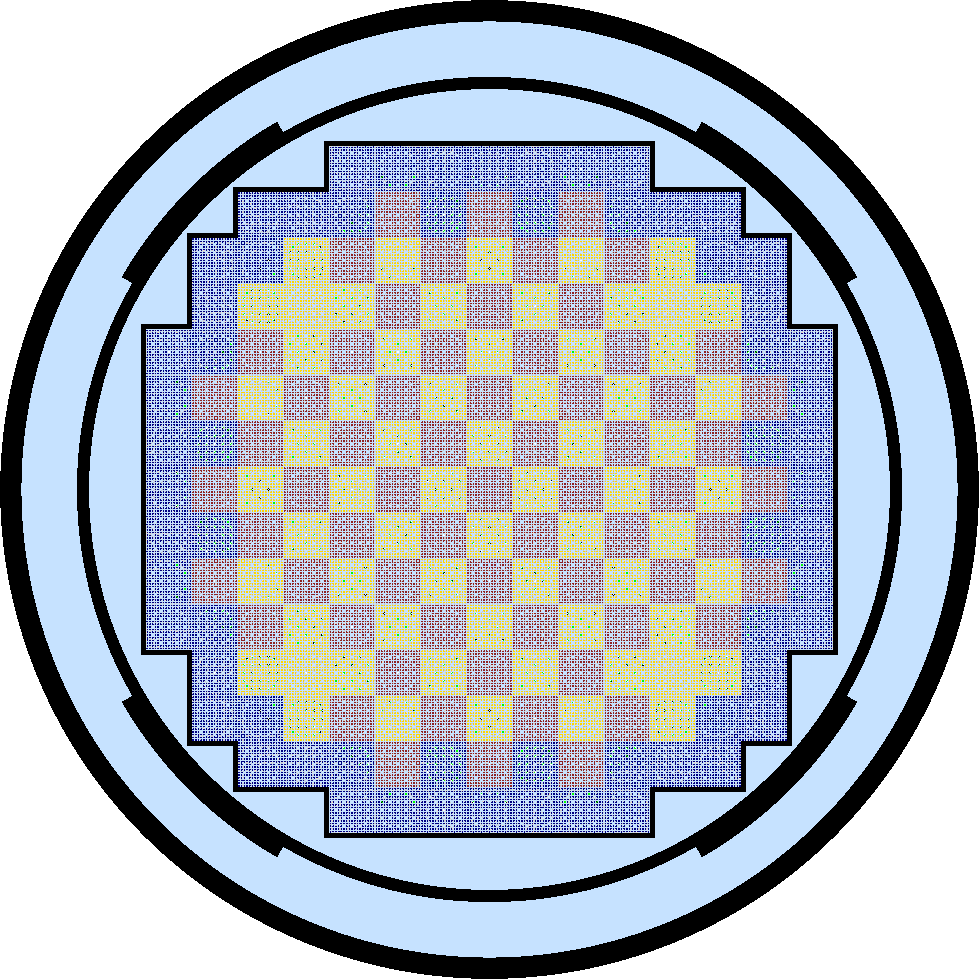
\includegraphics[width=5in]{figures/core.png}};
        \begin{scope}[every node/.style={draw,red,ultra thick,minimum width=\wwl,minimum height=\wwl}]
          % draw domain boundaries
          \foreach \x in {0,...,\nn}
          {
            \foreach \y in {0,...,\nn}
            {
              \node (\x\y) at ($(core.center) + (\x*\wwl,\y*\wwl) - (\wwl*3,\wwl*3)$){};
            }
          }
        \end{scope}

      \end{tikzpicture}
    }
    \newlength{\wwly}
    \setlength{\wwly}{0.9543568464in}
    \newlength{\wwlyt}
    \setlength{\wwlyt}{0.4771784232in}
    \newlength{\wwlyf}
    \setlength{\wwlyf}{0.09543568464in}
    \scalebox{0.5}{
      \begin{tikzpicture}
        \fill[white] (-2.5in,-2.5in) rectangle (2.5in,2.5in);
        \node[inner sep=0,opacity=0.5] (core)
          {\includegraphics[width=4.771784232in]{figures/row_8_mats_axial_grids_enhanced.png}};

%        \begin{scope}[every node/.style={draw,blue,minimum width=\wwl,minimum height=\wwlyf}]
%          % draw domain boundaries
%          \foreach \x in {0,...,\nn}
%          {
%            \foreach \y in {0,...,49}
%            {
%              \node (\x\y) at ($(core.center) + (\x*\wwl,\y*\wwlyf) - (\wwl*3,\wwlyf*24.5)$){};
%            }
%          }
%        \end{scope}

        \begin{scope}[every node/.style={draw,red,ultra thick,minimum width=\wwl,minimum height=\wwlyt}]
          % draw domain boundaries
          \foreach \x in {0,...,\nn}
          {
            \foreach \y in {0,...,9}
            {
              \node (\x\y) at ($(core.center) + (\x*\wwl,\y*\wwlyt) - (\wwl*3,\wwlyt*4.5)$){};
            }
          }
        \end{scope}

%        \begin{scope}[every node/.style={draw,red,ultra thick,minimum width=\wwl,minimum height=\wwly}]
%          % draw domain boundaries
%          \foreach \x in {0,...,\nn}
%          {
%            \foreach \y in {0,...,4}
%            {
%              \node (\x\y) at ($(core.center) + (\x*\wwl,\y*\wwly) - (\wwl*3,\wwly*2)$){};
%            }
%          }
%        \end{scope}
      
      \end{tikzpicture}
    }

    \caption{Geometry of the BEAVRS PWR benchmark showing one of the domain
    meshes used for large-scale depletion tally runs. Domains were sized to
    exactly fit a 3x3 group of assemblies radially. \emph{Left:} Radial top-down
    view. \emph{Right:} Axial view, showing 10 domains.\label{fig:depl_mesh}}
\end{figure} 

The full depletion problem was studied with OTF memory management, for the
scenarios in Table~\ref{tbl:depletion_meshes}. As shown in
Figure~\ref{fig:depl_mesh}, all cases were run with a domain mesh sized radially
to exactly fit a 3x3 section of fuel assemblies, and with axial refinements as
needed to accommodate the maximum local memory burden. Timing results are
presented in Table~\ref{tbl:depletion_tallies}. These results show particle
tracking rates consistent with those observed for non-DD Monte Carlo tallies
with similar complexity. For instance, non-DD runs using the same tally
parameters over a simple pin mesh were also observed to spend 7 times longer in
active tally batches than inactive batches.

\begin{table}
  \begin{center}
    \caption[Full-core depletion test scenarios]{Full-core depletion scenarios
    run for the BEAVRS geometry, with varying levels of spatial discretization
    and tally refinement. Nuclides for depletion were drawn from an ORIGEN-S
    V\&V report \cite{nuclides206}. \label{tbl:depletion_meshes}}
    \begin{tabular}{ccrrcrr}
    \toprule
    Case & 
    \pbox{20cm}{Rings \\ per Pincell} & 
    \pbox{20cm}{Axials \\ per Pincell} & 
    \pbox{20cm}{Number \\ of Nuclides} & 
    \pbox{20cm}{Number \\ of Scores} & 
    \pbox{20cm}{Total No. of \\ Tallies (M)} & 
    \pbox{20cm}{Total \\ Memory (GB)} \\
    \midrule
1 & 10 & 25 & 1 & 1 & 12.738 & 0.2847 \\
2 & 10 & 50 & 1 & 1 & 25.476 & 0.5694 \\
3 & 10 & 100 & 1 & 1 & 50.952 & 1.139 \\
 & & & & & & \\
4 & 10 & 25 & 206 & 1 & 12.738 & 58.65 \\
5 & 10 & 50 & 206 & 1 & 25.476 & 117.3 \\
6 & 10 & 100 & 206 & 1 & 50.952 & 234.6 \\
 & & & & & & \\
7 & 10 & 25 & 206 & 6 & 12.738 & 351.9 \\
8 & 10 & 50 & 206 & 6 & 25.476 & 703.8 \\
9 & 10 & 100 & 206 & 6 & 50.952 & 1408 \\
    \bottomrule
    \end{tabular}
  \end{center}
\end{table}

\begin{table}
  \begin{center}
    \caption[OTF tally timing results for terabyte tally BEAVRS
    runs]{Timing results in seconds for full-core tallies with the depletion
    mesh scenarios in Table~\ref{tbl:depletion_meshes}. $I$: Initialization
    time; $B_i$: Time in inactive batches; $B_a$: Time in active batches $F$:
    finalization time; $T$: total run time. All runs were carried out with 5
    active and 5 inactive batches, used 1 process per domain, and did not employ
    load balancing. All domain meshes used 7x7 domains radially as shown in
    Figure~\ref{fig:depl_mesh}, with a varying number of axial domains. The
    total particles per batch were set to 1000 per process (\emph{i.e.} 2.45M
    particles per batch were used for the largest run).
    \label{tbl:depletion_tallies}}
    \begin{tabular}{ccccrrrrrr}
    \toprule
    Case & \pbox{20cm}{Number of \\ Axial Domains} & $I$ & $B_i$ & $B_a$ & $B_i/B_a$ & $F$ & $T$ \\
    \midrule
1 & 5 & 86 & 407 & 1057 & 2.60 & 6 & 1550 \\
2 & 5 & 124 & 509 & 1783 & 3.50 & 12 & 2415 \\
3 & 5 & 220 & 761 & 3949 & 5.19 & 23 & 4931 \\  
 & & & & & & & \\
4 & 5 & 96 & 407 & 1151 & 2.82 & 7 & 1654 \\
5 & 5 & 134 & 510 & 1915 & 3.75 & 13 & 2560 \\
6 & 5 & 248 & 764 & 4198 & 5.49 & 26 & 5211 \\
 & & & & & & & \\
7 & 10 & 93 & 402 & 2607 & 6.49 & 6 & 3102 \\
8 & 10 & 144 & 504 & 3571 & 7.08 & 12 & 4219 \\
9 & 50 & 554 & 825 & 6269 & 7.6 & 27 & 7648 \\
    \bottomrule
    \end{tabular}
  \end{center}
\end{table}

%\begin{figure}
%    \centering
%    \includegraphics[width=5in]{figures/depletion.pdf}
%    \caption[Active vs inactive calculation rate for full depletion
%    tallies]{Active vs inactive calculation rate for full depletion
%    tallies. \label{fig:active_inactive}}
%\end{figure}

This indicates that the OTF memory management used during DD runs is not a
significant source of overhead. Indeed, as confirmed by the results in
Figure~\ref{fig:otf_perf}, the OTF memory management scheme does not degrade
domain decomposition performance or impede the ability to load-balance with the
resource-matching strategy.


%% Results for OTF
\begin{figure}[h!]
    \centering
    \includegraphics[width=0.45\textwidth]{figures/otf_domain_scale.pdf}
    \includegraphics[width=0.45\textwidth]{figures/otf_nodes_scale.pdf}
    \caption{Domain decomposition overhead with OTF materials and tallies for 1
    cell per BEAVRS fuel pin. \emph{Left}: Scaling with cubic domains over the
    geometry. \emph{Right}: Load balancing via resource matching on the 7x7x5
    domain mesh shown in Figure~\ref{fig:depl_mesh}. \label{fig:otf_perf}}
\end{figure}

%%%%%%%%%%%%%%%%%%%%%%%%%%%%%%%%%%%%%%%%%%%%%%%%%%%%%%%%%%%%%%%%%%%%%%%%%%%%%%%%
\subsection*{Number of Domains}

The number of domains chosen for each case in the full run made use of a
heuristic for choosing domain decomposition parameters. Specifically, the
portion of total tally and material memory that would be assigned to any compute
node must fit into local available memory on that node. For this analysis, it
is straightforward to calculate the total memory needed for materials and
tallies in PWR problems as

\begin{equation}
  \begin{aligned}
    M =& M_{materials} + M_{tallies} \\
    =& P C I m_m + P C I S m_t \\
    =& P C I \left(m_m + S m_t\right)
  \end{aligned}
  \label{eqn:mem_req}
\end{equation}

\noindent where $P$ is the number of fuel pins, $C$ is the number cells per fuel
pin (\emph{e.g.}, from rings and axial sections), $I$ is the number of isotopes
in the fuel, $S$ is the average number of scores needed for depletion, and $m_m$
and $m_t$ are the number of bytes needed for each nuclide atom density and tally
scoring bin, respectively.

Then, if the tally and material memory is divided equally among all domains, the
number of domains $N$ should be set by

\begin{equation}
  \begin{aligned}
    N \ge \frac{M}{M_{node} - M_{OS} - M_{metadata} - M_{XS}}
  \end{aligned}
  \label{eqn:mem_req}
\end{equation}

\noindent where $M_{node}$ is the installed memory on the node, $M_{OS}$ is the
memory overhead required by the operating system, $M_{metadata}$ is the memory
required to carry out the simulation (\emph{i.e.}, geometry data structures, OTF
maps, particle and fission bank arrays, etc.), and $M_{XS}$ is the memory
required for cross section data.

Of course, this will need to be adjusted accordingly if domains will be
irregularly-sized or materials and tallies are not regularly distributed across
domains.

%%%%%%%%%%%%%%%%%%%%%%%%%%%%%%%%%%%%%%%%%%%%%%%%%%%%%%%%%%%%%%%%%%%%%%%%%%%%%%%%
%%%%%%%%%%%%%%%%%%%%%%%%%%%%%%%%%%%%%%%%%%%%%%%%%%%%%%%%%%%%%%%%%%%%%%%%%%%%%%%%
\newpage
\section*{Conclusions}

Domain decomposition has been implemented in Monte Carlo neutron transport
methods several times in the literature, but it has never before been
demonstrated to successfully handle the full scale reactor problem. Instead it
has been regarded with pessimism, with Brown stating that such an approach is
``doomed to fail'' on future systems due to particle communication and load
imbalance inefficiencies \cite{forrest_mc_prospects}.

This thesis adds to the small but growing body of work that challenges this
conventional wisdom, contributing the following:

\begin{itemize}
  \item Domain decomposition algorithms
  \begin{itemize}
    \item Efficient and scalable inter-domain particle communication logic
    \item On-the-fly tally and material data management logic
    \item Efficient intra-domain OTF tally reduction logic
    \item Random number reproducibility logic in all routines
  \end{itemize}
  \item Load balancing
  \begin{itemize}
    \item Investigations of Monte Carlo load balancing strategies
    \item Analyses of the resource-distribution load-balancing strategy
  \end{itemize}
  \item Modeling
  \begin{itemize}
    \item Updated performance models for particle communication and load
    imbalance penalties
    \item Performance models for the resource-distribution load balancing strategy
    \item Heuristics for choosing decomposition parameters
  \end{itemize}
  \item Demonstrations and predictions for PWR problems
  \begin{itemize}
    \item Performance model predictions showing overhead no more than a factor
    of four for fine domain meshes
    \item Simulation results showing low-effort load balancing strategies
    almost completely eliminating parallel inefficiencies from imbalanced
    workloads
    \item Simulation results of a full-core PWR problem with realistic
    depletion material and tally memory burdens showing particle tracking rates
    comparable with non-domain-decomposed simulations
  \end{itemize}
\end{itemize}

This work makes progress towards enabling Monte Carlo methods for application
to high-fidelity simulations of nuclear reactors. Specifically, it has been
demonstrated that the intense tally and material memory burden can been
addressed with domain decomposition without significant overhead over non-DD
simulations, especially if load-balancing strategies are employed.

As shown in Figures~\ref{fig:imbal_removed} and~\ref{fig:otf_perf}, if load
imbalances are addressed with the resource-matching strategy \textbf{we expect
domain-decomposed Monte Carlo simulations of PWRs to take between 1.4x and 1.75x
as long as the equivalent non-DD runs}.

\newpage
%%%%%%%%%%%%%%%%%%%%%%%%%%%%%%%%%%%%%%%%%%%%%%%%%%%%%%%%%%%%%%%%%%%%%%%%%%%%%%%%
\subsection*{Performance Predictions}

Full-scale analyses will differ from the runs carried out in this work
primarily in the total number of particle histories run to achieve good
statistical convergence of tallies. This thesis confirms the parallel efficiency
of domain decomposition, thus estimates for run times can be obtained using
observed per-processor particle tracking rates as the total amount of work is
divided among many compute nodes.

For instance, results from the largest run presented in
Table~\ref{tbl:depletion_tallies} indicate an aggregate particle tracking rate
of 1.25 seconds per particle during active batches. Thus if \ul{10~billion
particle histories} are to be simulated with the current version of OpenMC
without load-balancing, almost 400 CPU-years would be required. Fortunately, the
situation is much improved when accounting for several practicalities of the
algorithm as well as of current and future supercomputing architectures.

First, the present DD implementation did not utilize shared memory parallelism
on each compute node: only one thread\footnote{``Threads'' are sequences of
programmed instructions fed to a processing unit often associated with
multi-tasking. Different \emph{software} threads can be executed by a single
processing unit that alternates back and for between them, whereas
\emph{hardware} threads are executed on separate processing units in parallel.}
per CPU tracked particles, which for the Titan Cray XK7 leaves 15 hardware
threads un-used on each CPU. Future HPC architectures are projected to have many
more hardware threads, but for current architectures we can conservatively
assume a 10x increase in particle tracking rates simply by making use of all
hardware threads available on a single CPU with shared memory parallelism (for
which efficient implementations have been previously demonstrated in OpenMC,
\emph{e.g.} by Siegel et al. in 2013 \cite{Siegel_multicore_openmc}). For the
purposes of estimation, this brings our particle tracking rate to 0.125
sec/particle and the time required for the large run to 40 CPU-years.

Second, given the relatively small number of domains needed (2450 for the
largest run in this work) compared to the number of available compute nodes on
HPC machines (projected to be $\sim1$M in 10 years), it will not be difficult to
distribute extra resources across domains to nearly eliminate load imbalances.
Since load imbalances were observed to be about a factor of four for this domain
mesh, this brings our particle tracking rate to 0.03125
sec/particle\footnote{This particle tracking rate is roughly consistent with
those reported by Romano in \cite{Romano201320} for the same supercomputer.} and
the time for the large run to 10 CPU-years.

This is manageable: \textbf{10,000 compute nodes} on Titan (a little over half
the machine) should complete this run in under \textbf{9 hours}. Without
decomposition, such a run was \ul{previously not achievable} for any amount of
simulation time. Furthermore, with these algorithms the situation should easily
continue to improve as the concurrency of HPC machines increases in the next
several years.


%Finally, it should be noted that the tally algorithms used in OpenMC were not
%optimized at all in this work, and that more efficient implementations exist in
%production codes, \emph{e.g.}, MC21 \cite{mc21_physor2014_beavrs}).

%%%%%%%%%%%%%%%%%%%%%%%%%%%%%%%%%%%%%%%%%%%%%%%%%%%%%%%%%%%%%%%%%%%%%%%%%%%%%%%%
\newpage
%\subsection*{Future Work}

%The present implementation addressed the major issues thought to stand in the
%way of efficient use of domain decomposition with Monte Carlo, but several items
%of future work remain:

%\begin{itemize}
%  \item More optimized algorithms
%  \begin{itemize}
%    \item More advanced particle buffering, \emph{e.g.} with
%    incorporation of the sparse and in-place schemes discussed by Felker et al.
%    in \cite{Felker04062012}
%    \item More streamlined I/O and post-processing routines
%    \item More efficient handling of cells cut by domain boundaries, including
%    automatic cell volume calculation/tallies
%  \end{itemize}
%  \item More optimized load balancing 
%  \begin{itemize}
%    \item ``Memory load balancing,'' \emph{i.e.}, some
%    combination of domain decomposition and data decomposition
%    \item Modifications to the inter-domain communication logic to enable
%    compute nodes to work on more than one low-workload domain
%    \item Adaptive mesh refinement and re-balancing during simulation, as
%    discussed by Procassini in \cite{Procassini} 
%  \end{itemize}
%\end{itemize}

%It should be noted that these items exclusively refer to domain decomposition.

%\begin{itemize}
%  \item More efficient tally implementation
%  \item More efficient shared-memory parallelism implementation
%\end{itemize}

%%%%%%%%%%%%%%%%%%%%%%%%%%%%%%%%%%%%%%%%%%%%%%%%%%%%%%%%%%%%%%%%%%%%%%%%%%%%%%%%
%%%%%%%%%%%%%%%%%%%%%%%%%%%%%%%%%%%%%%%%%%%%%%%%%%%%%%%%%%%%%%%%%%%%%%%%%%%%%%%%
% BIBLIOGRAPHY

\begin{singlespace}
\bibliographystyle{ans}
\bibliography{references}
\end{singlespace}

\end{document}
